%================================================
%	PACKAGES AND THEMES
%================================================
\documentclass[t,aspectratio=169,xcolor=dvipsnames]{beamer}

\usetheme{SimplePlusAIC}

\usepackage{hyperref}
\usepackage{graphicx} % Allows including images
\usepackage{booktabs} % Allows the use of \toprule, \midrule and  \bottomrule in tables
\usepackage{svg} % Allows using svg figures
%\usepackage{makecell}
\newcommand*{\defeq}{\stackrel{\text{def}}{=}}
\usepackage{setspace}
\usepackage[T1]{fontenc}
\usepackage{helvet}
%\usepackage{textgreek}
\usepackage{amsmath}
\usepackage{bm}
\usepackage{ragged2e}
\usepackage{xfrac}
% \usepackage[nice]{nicefrac}
\usepackage[loose]{units}
%\usepackage{braket}
%\usepackage{gensymb}
% \usepackage[cm]{sfmath}
%\usepackage{verbatim}
%\usepackage{fancyvrb}
\usepackage{tikz} % Allows nice main page with logo

%\setbeamertemplate{blocks}[rounded][shadow] % block options

\usepackage[svgnames,table]{xcolor}
\arrayrulecolor{black}
\setlength{\arrayrulewidth}{0.20mm}
\renewcommand{\arraystretch}{1.40}  % stretch tables row size

%================================================
%	TITLE PAGE
%================================================
\title[short title]{Le chapitre français du CAA} 
\subtitle{\textit{Computer Applications and Quantitative Methods in Archaeology} -- CAA-FR}

\author{https://caafrance.hypotheses.org}
% \institute[CBI]{Center for Anything, Department of Something \\ University of Anywhere \\ Somewhere \\ ~ \\}

\date{\textcolor{nyublue}{GMPCA 2025, Rouen, 14 avril 2025}}

%================================================
%	BEGIN DOCUMENT 
%================================================
\begin{document}

%------------------------------------------------
%	TITLE SLIDE
%------------------------------------------------
\begin{frame}[plain]

    \titlepage
    
\end{frame}

%------------------------------------------------
%	OUTLINE SLIDE
%------------------------------------------------
% \begin{frame}[plain]

%     \frametitle{OUTLINE} 
%     \framesubtitle{~}

%     \begin{spacing}{1.2}
%         \tableofcontents
%     \end{spacing}
    
% \end{frame}

%~~~~~~~~~~~~~~~~~~~~~~~~~~~~~~~~~~~~~~~~~~~~~~~~
% \section{CAA-Int and CAA-FR}
%~~~~~~~~~~~~~~~~~~~~~~~~~~~~~~~~~~~~~~~~~~~~~~~~

%~~~~~~~~~~~~~~~~~~~~~~~~~~~~~~~~~~~~~~~~~~~~~~~~
% \subsection{Subsection 1}
%~~~~~~~~~~~~~~~~~~~~~~~~~~~~~~~~~~~~~~~~~~~~~~~~

%------------------------------------------------
%	NEW SLIDE
%------------------------------------------------
\begin{frame}{overview caa-int}

    \frametitle{The CAA International} 
    %\framesubtitle{National Chapters of the CAA-Int.}

    \vspace{0.5mm}

    \begin{figure}
        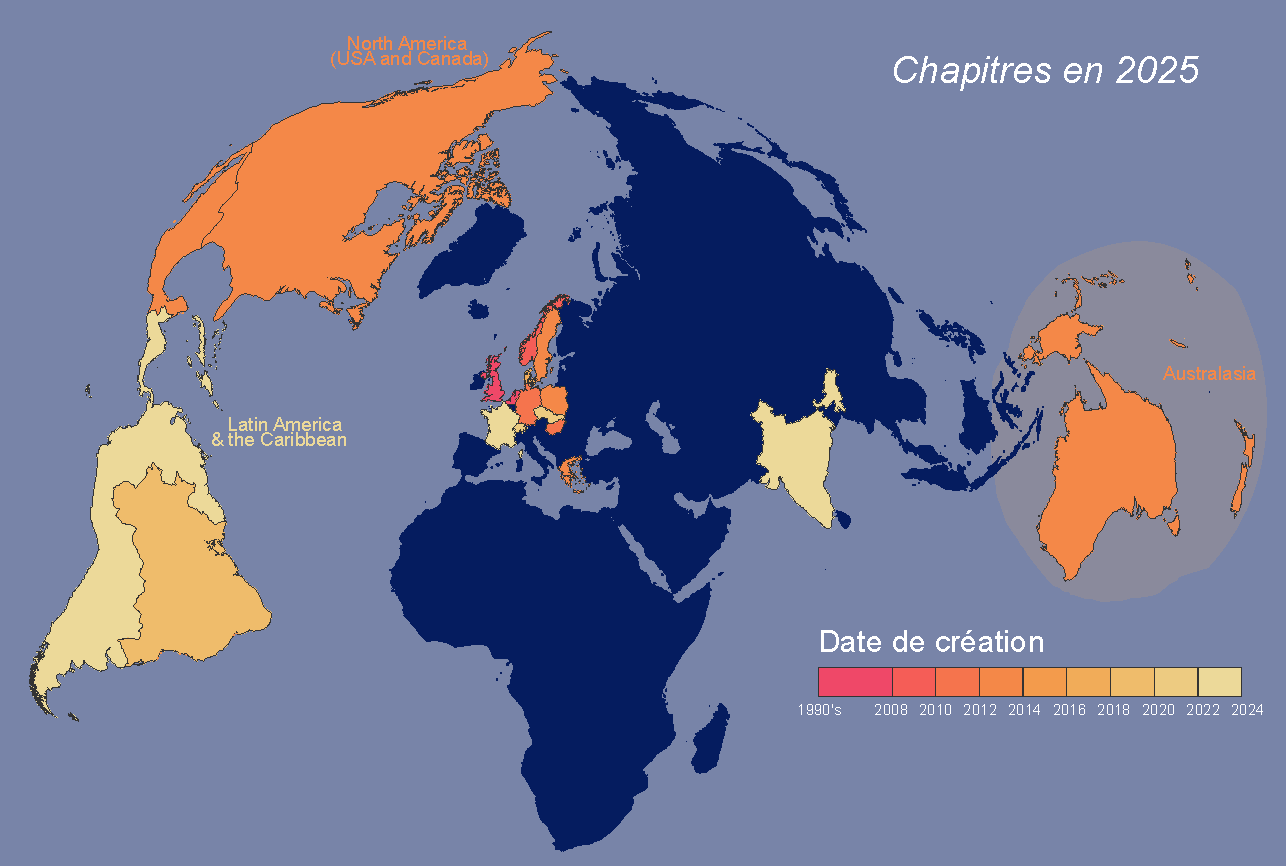
\includegraphics[height=0.8\textheight]{figures/national-chapters_2025.pdf}
    \end{figure}

\end{frame}

%~~~~~~~~~~~~~~~~~~~~~~~~~~~~~~~~~~~~~~~~~~~~~~~~
% \subsection{Subsection 2}
%~~~~~~~~~~~~~~~~~~~~~~~~~~~~~~~~~~~~~~~~~~~~~~~~

% %------------------------------------------------
% %	NEW SLIDE
% %------------------------------------------------
% \begin{frame}

%     \frametitle{CAA International} 
%     \framesubtitle{National Chapters of the CAA-Int.}

%     \vspace{-2mm}

%     \begin{columns}[t] 

%         \column{0.47\textwidth} 

%         \textbf{Bold text 1}
        
%         \begin{itemize}        
%             \item Aaaa
%             \item Bbbb
%             \item Cccc
%         \end{itemize}

%         \vspace{10mm}
        
%         \begin{figure}
%             \centering
%             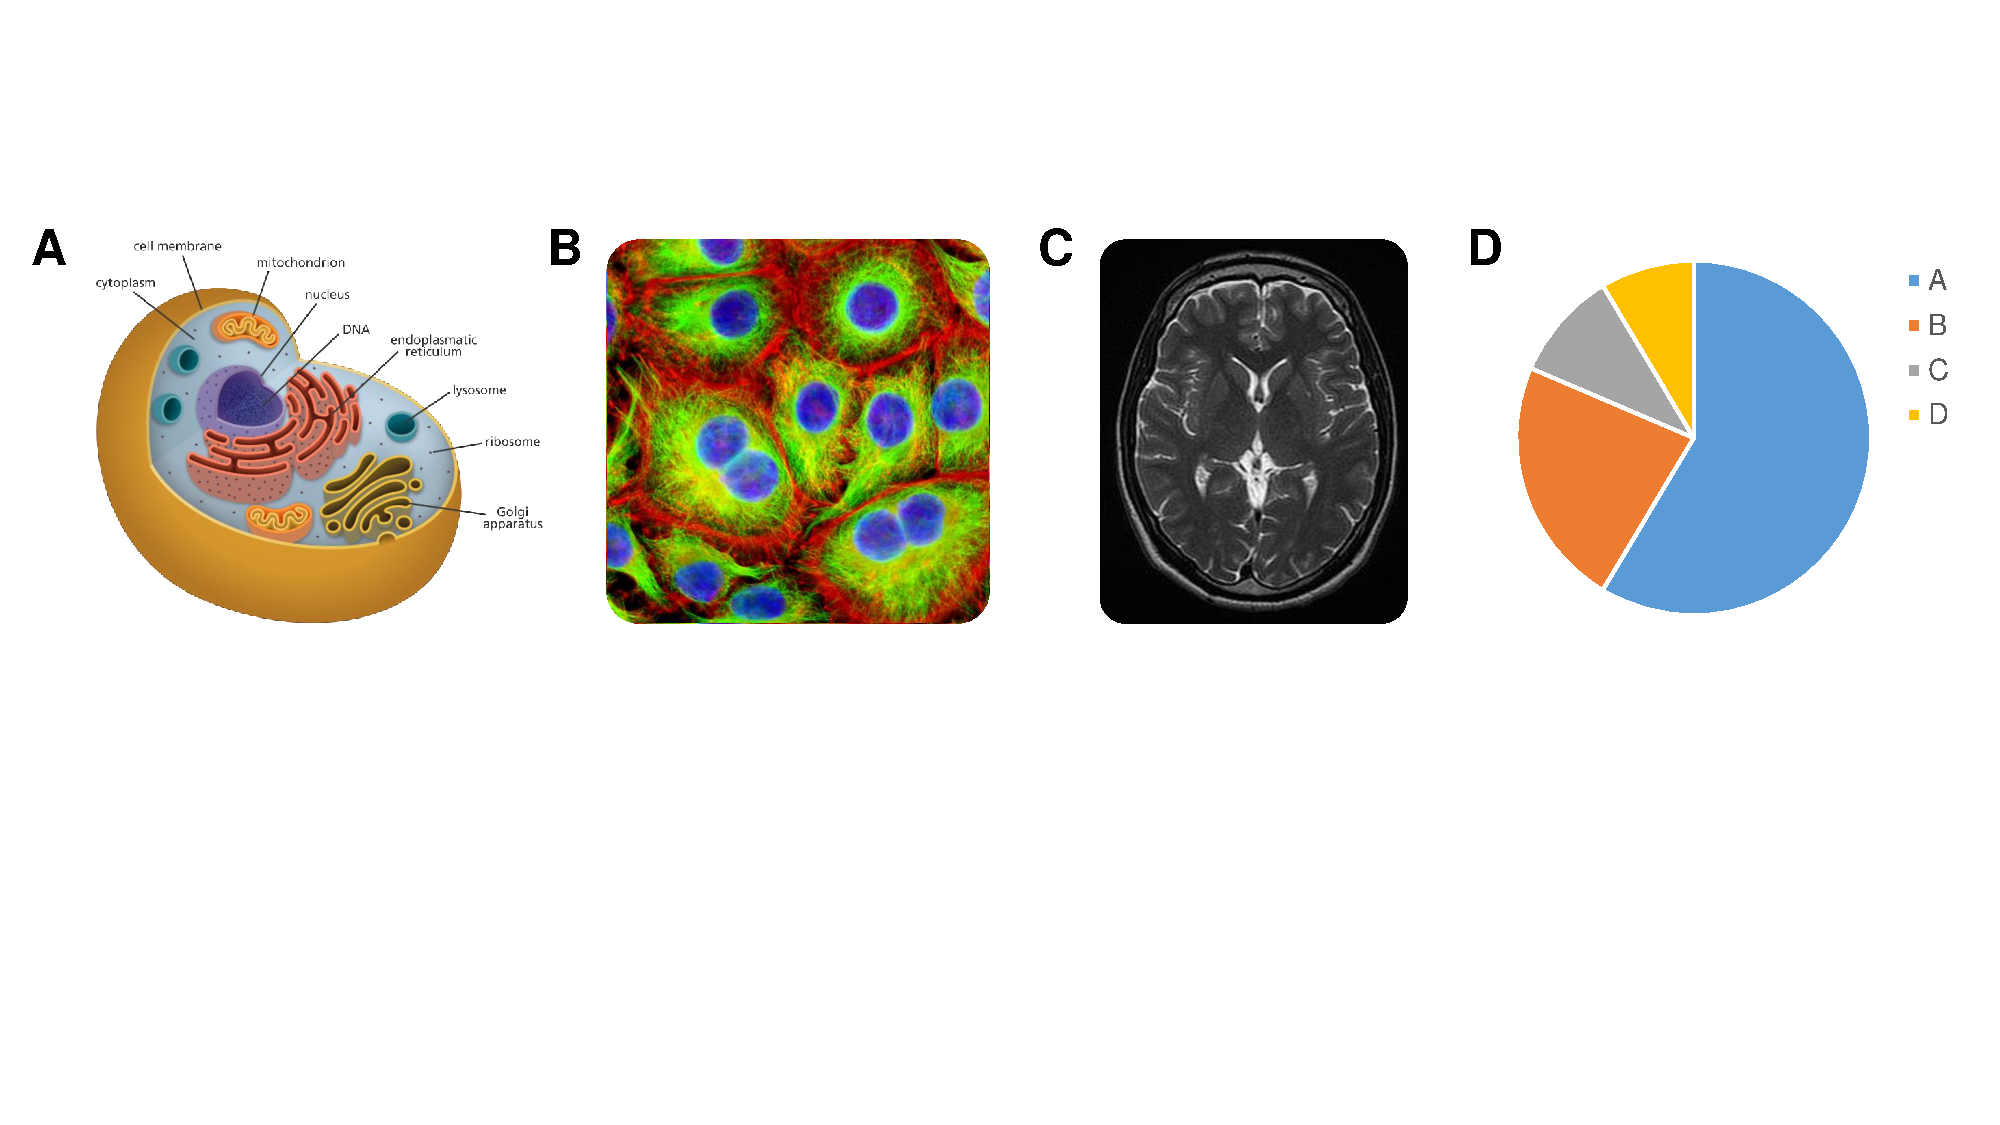
\includegraphics[width=0.9\linewidth]{figures/fig_example_1.pdf}
%         \end{figure}
      
%         \column{0.47\textwidth}

%         \textbf{Bold text 2}
        
%         \begin{itemize}        
%             \item Aaaa (\textbf{A})  
%             \item Bbbb (\textbf{B})
%         \end{itemize}

%         \vspace{-30mm} 
        
%         \begin{figure}
%             \hspace{30mm}
%             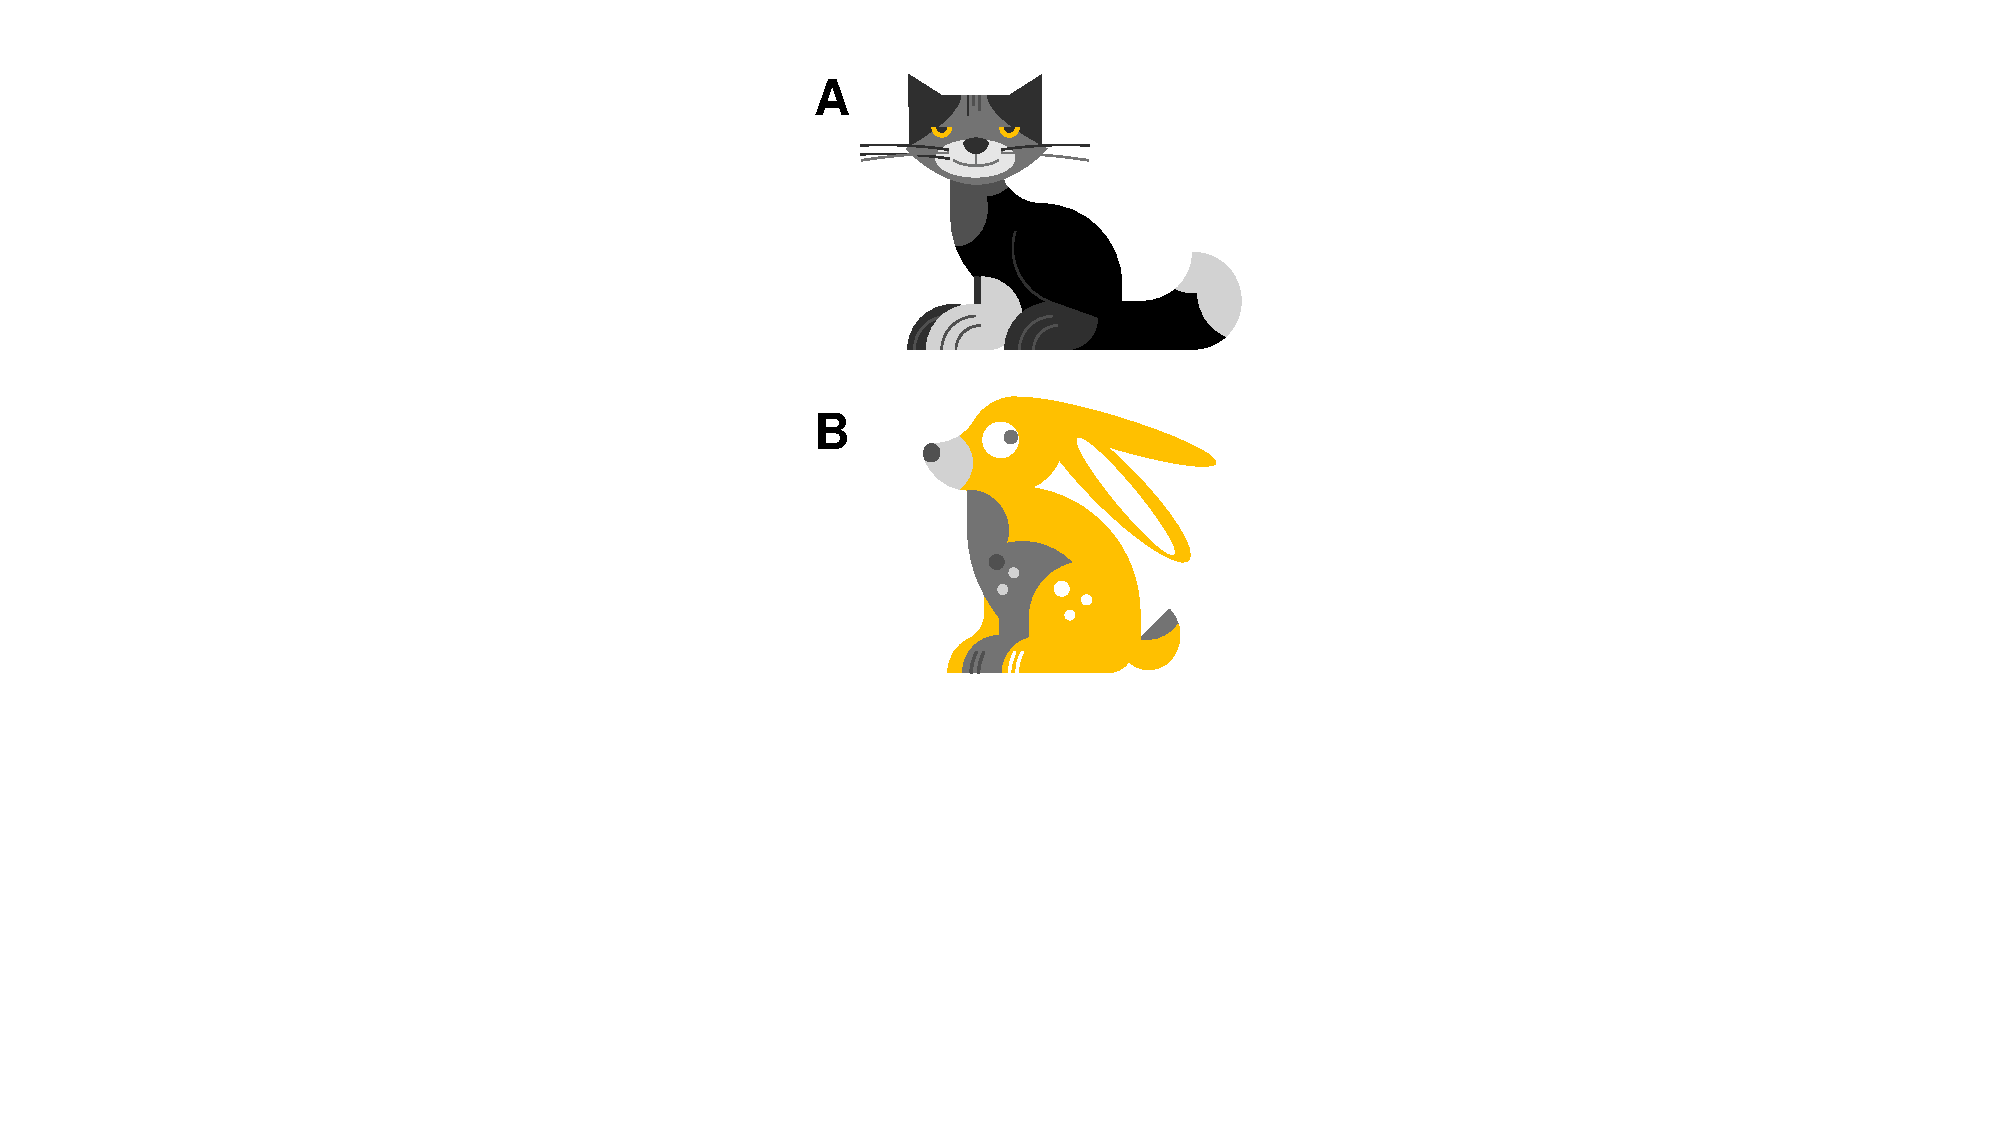
\includegraphics[width=0.50\linewidth]{figures/fig_example_2.pdf}
%         \end{figure}

%     \end{columns}

% \end{frame}


\begin{frame}{overview caa-fr 1}

    \frametitle{Overview of the CAA-FR} 
    %\framesubtitle{Overview}

    % \vspace{-2mm}

    \begin{block}{\textbf{Creation and Objectives}}
       
        \begin{itemize}
            \item \textbf{2024}: Creation during CAA Conference in Auckland
            \item To bring together archaeologists, archaeometrists, mathematicians, computer scientists and members of other disciplines based in France to complement and extend the interests of CAA International
            \item To encourage communication between these disciplines
            \item To give a survey of present work in the field
            \item To stimulate discussion and future progress in the application of information technology to archaeological research and practice
            \item To provide guidance and support in the form of seminars and/or workshops
        \end{itemize}

    \end{block}

    \end{frame}

    \begin{frame}{overview caa-fr 2}

    \frametitle{Overview of the CAA-FR} 
    %\framesubtitle{Overview}
        \begin{block}{\textbf{Current \textit{Bureau}}}
       
        \begin{itemize}
            \item \textbf{2024-2025} \& an election biennially at the CAA-FR General Meeting
            \item \textbf{Three speakers}: Dr Nicolas Frerebeau (UMR 6034 Archéosciences Bordeaux), Dr Sébastien Plutniak (UMR 7324 CITERES), Dr Gwénaëlle Moreau (SpaceARC).% j'ai fait du copier-coller, si ça tient à moi > je virerai le "Dr"
            \item \textbf{Three vice-speakers}: Dr Anaïs Vignoles (MSCA fellow), Mathias Bellat (PhD candidate, University of Tübingen), Dr Julie Gravier (UMR 6049 ThéMA)
        \end{itemize}

    \end{block}
    
    \end{frame}

    % \begin{exampleblock}{\textbf{Example Block title}}

    %     \begin{enumerate}
    %         \item \textbf{Item 1:} Aaaa
    %         \item \textbf{Item 2:} Bbbb
    %         \begin{enumerate}[a.]
    %             \item \textbf{Item 3:} Cccc   
    %             \item \textbf{Item 4:} Dddd 
    %         \end{enumerate}
    %     \end{enumerate}

    % \end{exampleblock}

%------------------------------------------------
%	NEW SLIDE
%------------------------------------------------
\begin{frame}{colloque ACQuA}

    \frametitle{Activities since 2024} 
    %\framesubtitle{Subtitle}

    \begin{alertblock}{\textbf{ACQuA Colloquium}}
       
        

    \end{alertblock}

\end{frame}

\begin{frame}{activities}

    \frametitle{Activities since 2024} 
    %\framesubtitle{Subtitle}

    \begin{alertblock}{\textbf{Since 2024}}
       
        \begin{itemize}
            \item \textbf{Item 1:}
            \item \textbf{Item 2:}
            \begin{itemize}
                \item \textbf{Item 3:} Cccc 
                \item \textbf{Item 4:} Dddd 
            \end{itemize}
        \end{itemize}

    \end{alertblock}

\end{frame}

%~~~~~~~~~~~~~~~~~~~~~~~~~~~~~~~~~~~~~~~~~~~~~~~~
% \section{Conclusion}
%~~~~~~~~~~~~~~~~~~~~~~~~~~~~~~~~~~~~~~~~~~~~~~~~

%~~~~~~~~~~~~~~~~~~~~~~~~~~~~~~~~~~~~~~~~~~~~~~~~
% \subsection*{Conclusion}
%~~~~~~~~~~~~~~~~~~~~~~~~~~~~~~~~~~~~~~~~~~~~~~~~

%------------------------------------------------
%	NEW SLIDE
%------------------------------------------------
% \begin{frame}

%     \frametitle{CONCLUSION} 
%     \framesubtitle{Subtitle}

%     \vspace{2mm}
    
%     \begin{spacing}{1.2} % more space between items

%     \begin{itemize}
    
%         \item \textbf{Conclusion 1:} Blablabla
        
%             \begin{itemize}
%                 \item \textbf{Item 1:} BloBloBlo \cite{dirac1974principles, einstein1935can}
%                 \item \textbf{Item 2:} Blublublu
%             \end{itemize}
            
%         \item \textbf{Conclusion 2:} Blablabla
        
%             \begin{itemize}
%                 \item \textbf{Item 1:} BloBloBlo
%                 \item \textbf{Item 2:} Blublublu
%             \end{itemize}         
        
%         \item \textbf{Conclusion 3:} Blablabla
        
%             \begin{itemize}
%                 \item \textbf{Item 1:} BloBloBlo \cite{feynman1948space}
%                 \item \textbf{Item 2:} Blublublu
%             \end{itemize}
            
%     \end{itemize} 

%     \end{spacing}

% \end{frame}

%------------------------------------------------
%	NEW SLIDE
%------------------------------------------------
% \begin{frame}[plain]

%     \frametitle{ACKNOWLEDGEMENTS} 
%     \framesubtitle{Thank you!}

%     \begin{columns}[t] 

%         \column{0.56\textwidth} 

%         \vspace{-1mm}
        
%         \begin{figure}
%             \centering 
%             
\includegraphics[width=0.35\linewidth]{logos/fig_logo_1.pdf}
%         \end{figure}

%         \vspace{-1mm}

%             \begin{columns}
    
%             \column{0.46\textwidth} 

%             {\small
            
%             \textbf{\textcolor{nyublue}{Collaborators}}\\
%             Aaaa Bbbb, PhD\\
%             Cccc Dddd, MD

%             ~

%             \textbf{\textcolor{nyublue}{NIH Grants}}\\
%             \textbf{R01} XX012345\\
%             \textbf{R21} XX678901\\

%             } % end footnotesize font

%             \column{0.46\textwidth} 

%             {\small
            
%             \textbf{\textcolor{nyublue}{Postdocs}}\\
%             Aaaa Bbbb, PhD (\textbf{A})\\
%             Cccc Dddd, MD

%             ~

%             \textbf{\textcolor{nyublue}{PhD Students}}\\
%             Aaaa Bbbb, PhD (\textbf{B})\\
%             Cccc Dddd, MD

%             }
    
%             \end{columns}
      
%         \column{0.36\textwidth}

%         \vspace{-14mm}

%         \begin{figure}
%             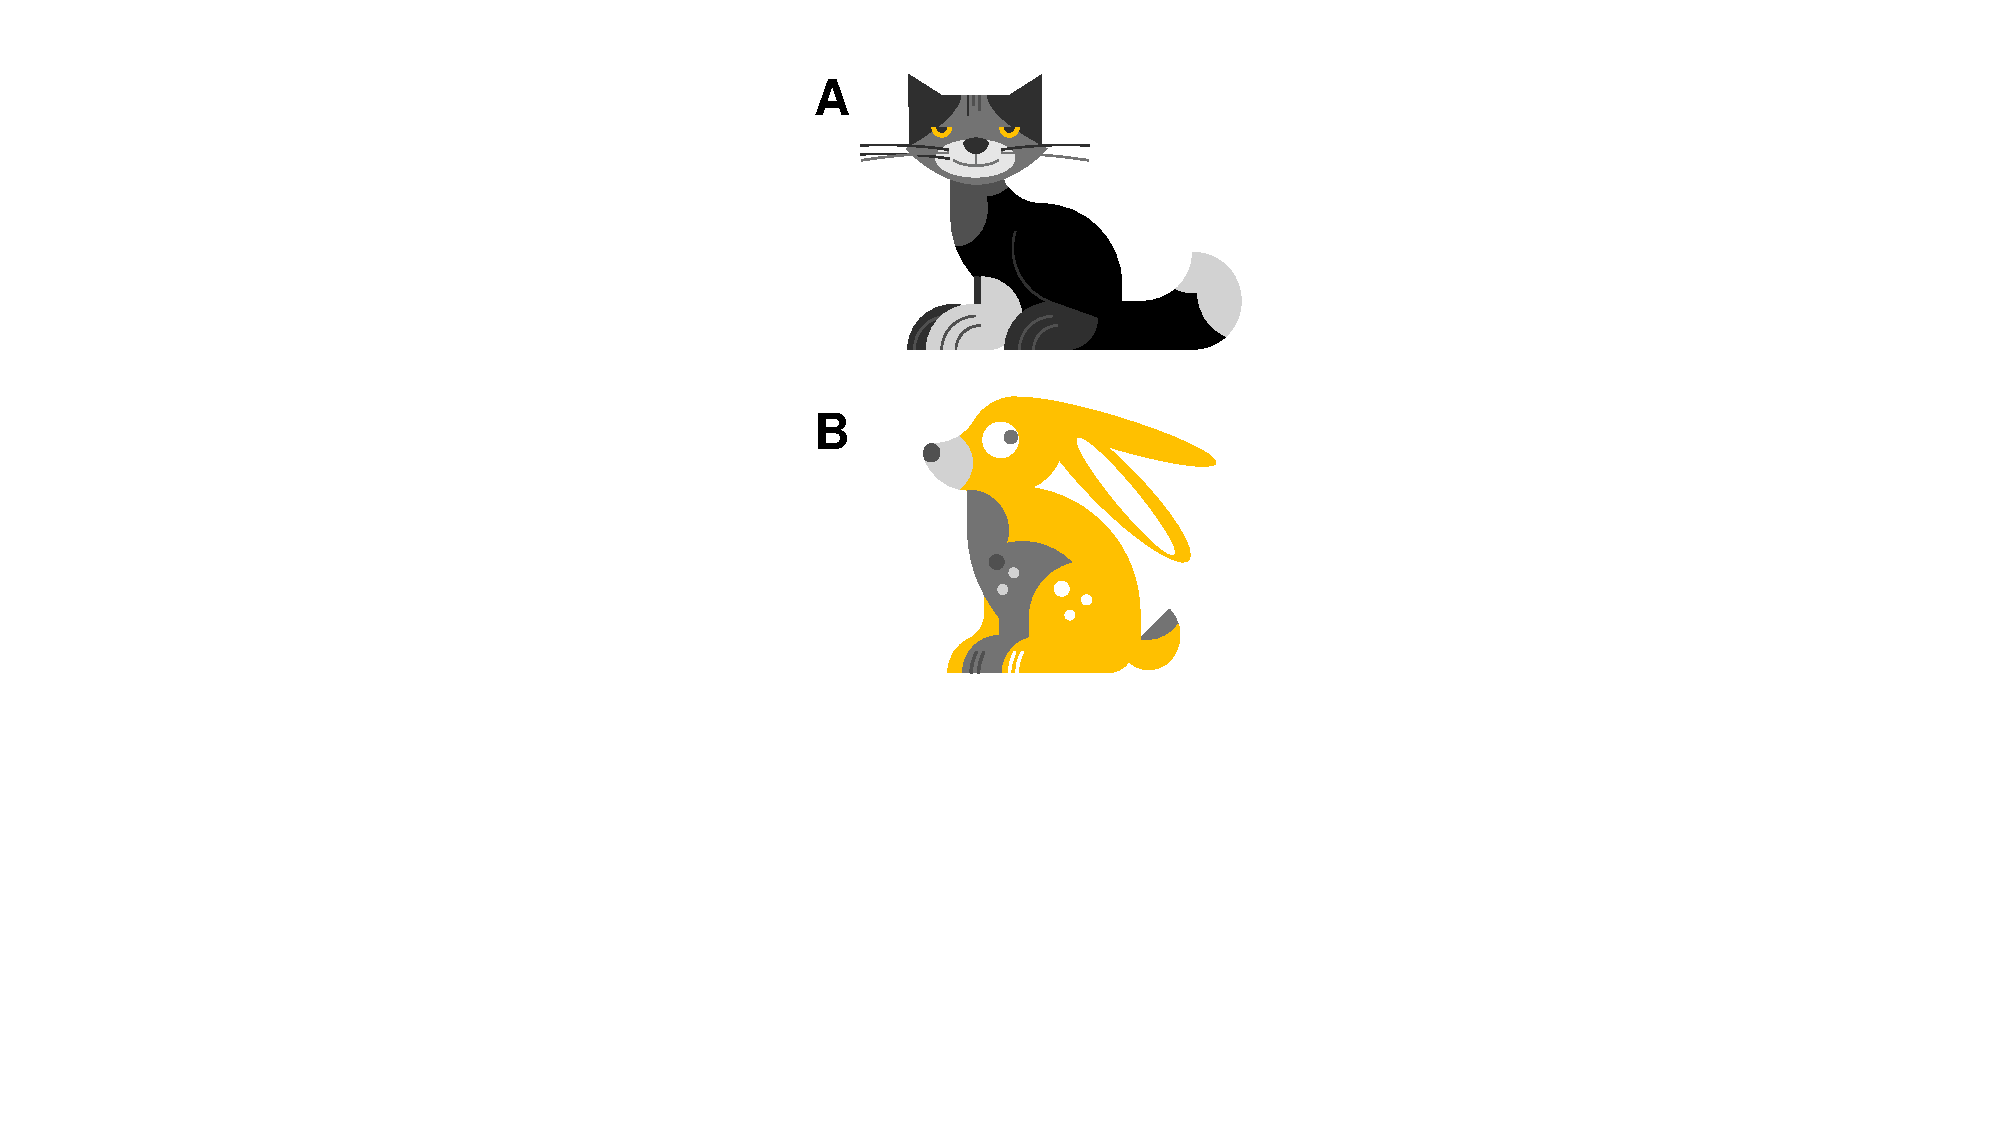
\includegraphics[width=1\linewidth]{figures/fig_example_2.pdf}
%         \end{figure}

%     \end{columns}

% \end{frame}



%================================================
%	END DOCUMENT 
%================================================
\end{document}
